\documentclass{standalone}
\usepackage{multicol}
\usepackage{tikz}
\usetikzlibrary{calc,angles,positioning,intersections,quotes,decorations.markings}
\usepackage{tkz-euclide}
\usetkzobj{all}
\usepackage{pgfplots}
\pgfplotsset{compat=1.16} 

\begin{document}
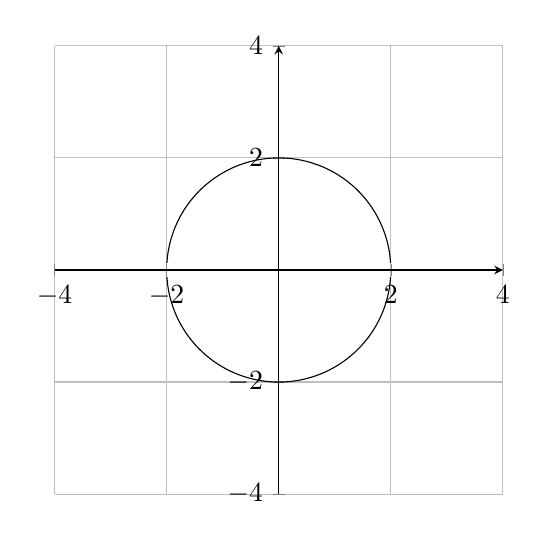
\begin{tikzpicture}
	\begin{axis}[axis lines=middle, axis equal image, grid=both, xmin=-4, xmax=4, ymax=4, ymin=-4, samples=790, mark=none]
		\addplot[mark=none]{sqrt(4-x^2)};
		\addplot[mark=none]{-sqrt(4-x^2)};
	\end{axis}
\end{tikzpicture}
\end{document}
